\documentclass[a4paper, openany]{memoir}

\usepackage[utf8]{inputenc}
\usepackage[T1]{fontenc} 
\usepackage[english]{babel}
\usepackage{amsmath}
\usepackage{amssymb}

\usepackage{booktabs}
\usepackage{fancyhdr}
\usepackage{float}
\usepackage{indentfirst}
\usepackage{graphicx}
\usepackage[linewidth=1pt]{mdframed}
\usepackage{multicol}
\usepackage{fancyvrb}

\pagestyle{fancy}
\fancyhf{}
\fancyhead[LE]{\leftmark}
\fancyhead[RO]{\rightmark}
\fancyhead[RE, LO]{PSD}
\fancyfoot[LE, RO]{\thepage}
\fancyfoot[RE, LO]{Pete Gautam}

\renewcommand{\headrulewidth}{1.5pt}

\chapterstyle{thatcher}
\setcounter{chapter}{3}

\begin{document}
\chapter{Requirements Management}
Requirements specify what a system should do. There are 2 types of requirements:
\begin{itemize}
    \item functional requirements, which describe actions that an actor can observe in practice.
    
    \item non-functional requirements, which describe properties of a system that an actor can observe in practice.
\end{itemize}
Design describes how a system does some task. A design is realised through an implementation. This is illustrated in the image below.
\begin{figure}[H]
    \centering
    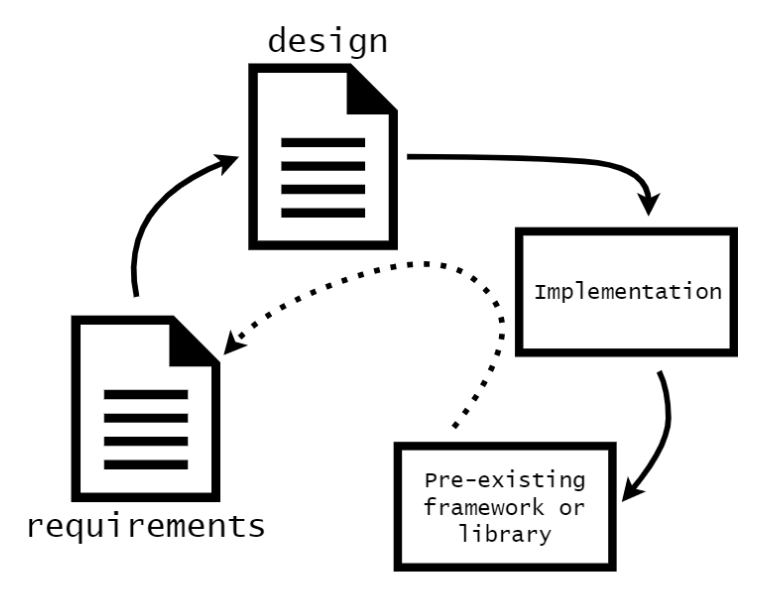
\includegraphics[scale=0.4]{src/requirements v design.PNG}
    \caption{Requirements, design and implementation.}
\end{figure}
\noindent We also need to consider pre-existing frameworks and libraries that the implementation may depend on. These might constrain what implementation options there are for a software system, which in turn constrains design and requirements. So, requirements should be considered with implementation.

Maintaining requirements as a project evolves is important. Requirements are the focus of the ongoing discussion with the customer to describe what the system should do. They also provide a basis for acceptance testing- we test the system so that it meets the requirements, and see which requirements have been realised in the implementation.

There are lots of different requirement-specific notations, such as:
\begin{itemize}
    \item formal specifications (mathematical notations, e.g. Z);
    \item viewframes;
    \item UML use cases and activity diagrams;
    \item pseudocode; and
    \item natural language.
\end{itemize}
There is a spectrum from formal specification to natural language. It is better to use the formal specification to drive acceptance testing- it has very precise specifications. However, it is harder to use formal specifications to negotiate with the customer- the customer needs to undergo training in order to understand the specification. On the other hand, it is better to use natural language to describe and negotiate with the customer, although it is often harder to use in acceptance testing since it is less precise and open to interpretation. User stories are commonly used in agile practices. It provides a semi-structured notation for describing requirements.

\section{Actors}
An actor (also called a role and a persona) describes the categories of the users that will perform actions on the system. We should avoid the user being too specific or too generic. It is used to partition the system into characteristic categories. It includes the actor's specific motivation for interacting with the system, i.e. their goals and current frustrations with the system.

Actors are essential for justifying the existence of features. Without an actor's motivation for a feature being in the system; such a feature is a waste to the system or even a defect. Actors can help to identify one of the types of system stakeholders to negotiate requirements with. For example, consider the following actor:
\begin{verbatim}
Name:           Elidth the Estate Agent
Goals:          Sell more houses (and get commission) by 
                securing more buyers and sellers for the agency.
Frustrations:   Customer can't register for themselves; 
                Unable to answer buyer questions on home visits.
\end{verbatim}
Note that a system actor need not be a human. We can use user stories to documenting actions performed by non-humans as well (e.g. another component in the software system). 

\section{User Stories}
We write user stories in the perspective of the user/actor. It follows the following format:
\begin{verbatim}
As an <actor>,
I want to <action on/by system> 
so that <rationale>.
\end{verbatim}
For example, the following is a user story:
\begin{verbatim}
As an estate agent,
I want to be motified about a new enquiry
so that I can follow up with a new client.
\end{verbatim}
Note that the rational given should not be circular. That is, the rational should not just restate the action; it should provide an independent justification.

\section{Requirements Scope}
In theory, every action on a system should have a user story. But, this means:
\begin{itemize}
    \item the scope of the requirements would be unbounded;
    \item many user stories would be duplicated across multiple systems- it may explain lots of details about the requirements;
    \item effort would be wasted on acceptance testing of underlying framework(s) and dependencies, which is not the aim of this project.
\end{itemize}
Instead, we should focus on business logic that is particular to the application under development. We can treat framework features as assumptions about user roles, e.g. we treat them as things that are given within each role.

We will now look at some user stories.
\begin{verbatim}
As a user,
I want to login
so that I can access privileged features.
\end{verbatim}
This is a bad user story. The user is not specified. The login feature is common, and usually provided by the underlying framework. Also, there is no real categorisation of goals and desires- it is generic and applies to every actor who wants to access the system. Instead, we should replace it with the following:
\begin{verbatim}
As an account owner,
I want to review a summary of my bank balances
so that I can monitor my cash flow.
\end{verbatim}
This is more business-specific for this project. Nonetheless, the generic user story might still be fine if the project is just for proof of concept. In that case, we can use the user story to demonstrate that the feature is available. So, these rules are not absolute- we need to judge what is appropriate as a user story depending on the context.

We can also use user stories for non-functional requirements, e.g.
\begin{verbatim}
As a lawyer,
I want my search properties to return in <5 seconds
so that I don't waste time.
\end{verbatim}
This is a performance requirement, not a functional requirement.

\section{Refining User Stories}
\subsection{Add more detail}
Along with the high-level descriptions for user stories, we can also refine them. We can add more detail. As we negotiate the requirements with the customer, we start adding details about different aspects to the implementation. For example, consider the following user story:
\begin{verbatim}
As a first time buyer,
I want to enquire about available properties that match 
my preferences
so that I can find somewhere to live.
\end{verbatim}
We can add the preferences included as time went on, e.g. budget, location, number of bedrooms, etc.

\subsection{User story tasks}
User stories must be refined into implementation tasks, e.g.
\begin{itemize}
    \item add search page to web front end;
    \item add search page to mobile app.
\end{itemize}
It is possible for user stories to share tasks.

\subsection{Story prioritisation- MOSCOW}
We can prioritise user stories/requirements using the MOSCOW system. The MOSCOW system can be used to rank the priorities of issues. We can assign each user story one of the following priorities:
\begin{itemize}
    \item Must have: these are critical features necessary for a system to work effectively. The software will not work without these or be usable.
    \item Should have: these are important features, but not critically essential without it. It makes the system more convenient. For example, bulk upload of files is a should have feature. It is possible to upload files one by one, but this makes uploading multiple files more efficient.
    \item Could have: these are niceties and stretch goals.
    \item Would be nice to have: these features are currently out of scope for the budget. These are potential features, but won't happen in this iteration.
\end{itemize}

\subsection{Estimating tasks}
Task estimation is useful, but difficult. In fact, some practitioners argue that estimation is fruitless. It is better to make short improvements before reviewing agenda. Sometimes, it is necessary for budgeting and wider planning. It helps identify poorly understood tasks and force their refinement/entertain. This helps reduce risk in project, even if the estimation is not accurate. It can help the team to understand what tasks they have to complete/what is involved in their implementation.

There are different methods for performing estimation:
\begin{itemize}
    \item Delphi methods: this is based on developing consensus.
    \item Market testing, price to win or bidding: the team announces a project and asks for bids to complete it and choose a bid (e.g. the lowest or the middle one) to be the estimate of the cost.
    \item Empirical methods, e.g. cocomo: we derive the cost of a task based on comparing it to similar projects.
    \item Algorithmic methods, e.g. function-point analysis: we analyse different features and likely properties of the task to be complete.
\end{itemize}

Planning poker is a Delphi method, and involves building consensus among the group. Each developer is asked to estimate a task with a card value and play that card independently. They then discuss the reason for the estimate before playing another round. The consensus is arrived at eventually. The cards describe story points- they describe how much a task is likely to take to implement. The estimates are project-specific, not person-specific. The higher the number, the longer it will take to implement.

We can measure story points and gets completed in a given period of time. We then attempt to translate the story point to personal-time estimate by measuring against the time it actually took (from previous experience). There are two extra cards:
\begin{itemize}
    \item ?, to mean that the task is too hard to estimate;
    \item coffee cup, to mean that they need to take a break.
\end{itemize}

\subsection{Scenario}
We can also use scenarios to refine user stories. They are useful for describing workflows, i.e. how a user story is realised. They can also be used for acceptance testing. It follows an arrange/act/assert flow, similar to a unit test. Its structure is:
\begin{verbatim}
Given <a fixture>
And <another fixture>
And <...>,
When <an action is performed on a feature>
And <another action is performed on a feature>
And <...>,
Then <a condition holds>
And <another condition holds>
And <...>.
\end{verbatim}
For example, the following is a scenario:
\begin{verbatim}
Given a mocked database of properties
And a property search API,
When a text search is performed for 29 Acacia Road,
Then Banana Man's property is returned.
\end{verbatim}
The workflow is described in a scenario. We start with the precondition, then look at the set of actions, and end up with the final outcomes.

\section{Storing user stories}
Some teams store their user stories as hand-written postcards stuck to a wall or whiteboard in the team space. It is easy to recognise and review as a whole, but hard to share across team locations. Moreover, it requires effort to maintain.

We can store user stores and tasks online. We should store user stories and scenarios as a text file within the version control tool. This is because requirements describe what the system should do. So, it should be stored alongside the implementation, which is what the system actually does. Tasks that realise the user story can be found in the issue tracker.

Tasks describe actions to be performed to make changes to the software system. User stories/scenarios describe what the system should actually do (whether it does it or not). This is also stored in the version control tool. This is a many-to-many relationship, i.e.
\begin{itemize}
    \item a user story might be realised by several task implementations; and
    \item a task may support the realisation of several user stories.
\end{itemize}

\section{INVEST}
We can ensure that user stories are of good quality by following the INVEST policy:
\begin{itemize}
    \item Independent: a user story should not depend on other user stories for realisation of a feature.
    \item Negotiable: there should be identifiable actor/class of actors with whom the user story can be refined;
    \item Valuable: it should be clear why the actor cares about the implementation in the user story;
    \item Estimable: it should be possible to estimate the user story. If it is not possible how long it will take to implement user story, it is a risk;
    \item Small: there should be small features that can be implemented independently;
    \item Testable: it should be possible to develop scenarios to describe the workflow to realise the user story has been implemented.
\end{itemize}

We will now look at some smelly stories and criticise them using the INVEST criteria. For example, consider the following user story.
\begin{verbatim}
As a user,
I want to search for properties
so that I can find properties.
\end{verbatim}
This story is not negotiable- it lacks an identifiable user. Moreover, it is not valuable- the rationale is circular. Next, consider the following story:
\begin{verbatim}
As an England cricket team fan,
I want to be notified of upcoming matches and be able to filter 
these notifications by match type (T20, 50-50, Test). Once I’ve 
been notified, I want to be able to retrieve all the match 
information, such as who is batting, what the score is, who is
bowling, how many overs have been bowled and so on. Once I’ve 
got the detailed view, I’d also like to be able to find out
about a player’s history, such as their batting statistics.
So that I can keep track of all that is going on with my 
favourite team.
\end{verbatim}
This user story is not small. Moreover, it is also not independent- there are many features bundled up inside the user story. We should break this into smaller, discrete, independent user stories which make them much easier to estimate. Finally, consider the following story:
\begin{verbatim}
As a driver,
I want passengers to wait at an agreed location
so that I can pick them up.
\end{verbatim}
This is not testable. It is beyond the scope of the software system to test/ensure this. The user story describes the behaviour of passengers, but it should describe the action that passengers can perform on the system. It is better if the system notifies the passengers of a collection point.

In summary, user stories are used to document the requirements, i.e. what should be implemented in a software system, and can used to track whether it is present or not. The key point is the requirements are basis of the negotiation. There are lots of ways of refining a user story to add more detail about what a system should do in order to support their implementation.

\end{document}